\chapter{Aufgabe 2}

\section{Teil 1}

\subsection{Sicherheitsziele}

Auch wenn im Szenario nicht explizit die \textbf{Verfügbarkeit} als direktes Sicherheitsziel des Online-Shops angegeben wurde, leiten wir dieses als indirektes Sicherheitsziel aus den Qualitätsansprüchen, wirtschaftlichen Zielen und den finanziellen Interessen des Online-Shop-Betreibers ab.\\
Besonders hervorzuheben sind folgende Sicherheitsziele, wobei eine grobe Klassifizierung der betroffenen Daten bzw. des Verantwortungsbereiches in Klammern erfolgt:

\begin{itemize}
    \itemsep0.5em
    \item \textbf{Vertraulichkeit} - vertrauliche Speicherung und Übermittlung von:
    \begin{itemize}
        \item Bestellungen (Vertragsdaten)
        \item Adresse und Bankverbindungen (Kundendaten)
    \end{itemize}
    \item \textbf{Integrität} - Schutz vor Manipulation
    \begin{itemize}
        \item der Datenbanken/Webanwendung, die den Datenbestand des Online-Shops beinhalten/anzeigen (Betreiber)
        \item der getätigten Bestellungen (Betreiber)
        \item des Webseiteninhalts zur Anzeige bei dem Anwender (Betreiber/Anwender)
    \end{itemize}
    \item \textbf{Authentizität / Verbindlichkeit}
    \begin{itemize}
        \item Bestellungen dürfen nicht abgestritten werden und müssen einem authentisierten Benutzer eindeutig zugeordnet werden können (Betreiber)
        \item verbindliche Zusicherung der Bestellungen an den authentisierten Benutzer (Betreiber)
    \end{itemize}
\end{itemize}

\subsection{Mögliche Bedrohungen}

Mit den angegebenen Sicherheitszielen sollen (nicht ausschließlich) die im Folgenden genannten Bedrohungen verhindert werden:


\begin{itemize}
    \itemsep0.5em
    \item \textbf{Vertraulichkeit}
    \begin{itemize}
        \item Abhören der Kommunikationsleitungen durch Malware an den Kommunikationsendpunkten (Rechner Nutzer / Server Betreiber) bzw. Zwischenstationen (Router, Firewallkomponenten)
    \end{itemize}
    \item \textbf{Integrität}
    \begin{itemize}
        \item Manipulation der \textit{Bestandsdaten} (Betreiber) durch Hintertüren, Malware, Social Engineering, \ldots
        \item Manipulation der \textit{übertragenen Daten} durch Man-in-the-middle-Angriffe, Umleiten von Anfragen, IP-Spoofing
    \end{itemize}
    \item \textbf{Authentizität / Verbindlichkeit}
    \begin{itemize}
        \item Tätigen von Bestellungen mit den Credentials authentisierter Nutzer / Nutzerdaten durch Dritte (User-Accounts, Kreditkarteninformationen)
        \item Umleiten von Bestellungen an Adressen Dritter mit Zahlungs-/Kundendaten authentisierten Nutzer
        \item Umleiten von Transaktionen an Dritte
    \end{itemize}
\end{itemize}

\subsection{Sicherheitsarchitektur}

Der Schutzbedarf des IT-Systems ist als \textit{hoch} einzustufen, bedingt durch die wirtschaftlichen Interessen des Betreibers sowie die sensiblen personenbezogenen Daten, die in den IT-Systemen des Betreibers gespeichert werden (Kontodaten, Adressdaten, \ldots).\\

Es sind Schutzmaßnahmen zu treffen, die nicht nur \textit{präventiv} wirken, sondern zur Wahrung der Sicherheitsqualität auch \textit{reaktiv} sowie \textit{detektiv}.

\subsubsection*{IT-System Betreiber}

Dem Betreiber wird empfohlen, zur Abwehr von Angriffen von Außen auf seine IT-Infrastruktur \textbf{Firewalls} in Form von \textbf{Paketfilter} und \textbf{Anwendungsproxies} einzusetzen, um sensible Daten durch maliziösen Internetverkehr abzuschirmen.\\
Hierfür eignet sich das in Abbildung~\ref{fig:screened_subnet} skizzierte \textbf{Screened Subnet mit Proxy Server} (\cite[89 f.]{ITS4}), bei dem in einer \textit{demilitarisierten Zone} die Webserver  des Online-Händlers betrieben werden, die durch \textbf{Paketfilter} auf den externen ``Anfragebedarf`` abgestimmt werden.\\

\begin{figure}
    \centering
    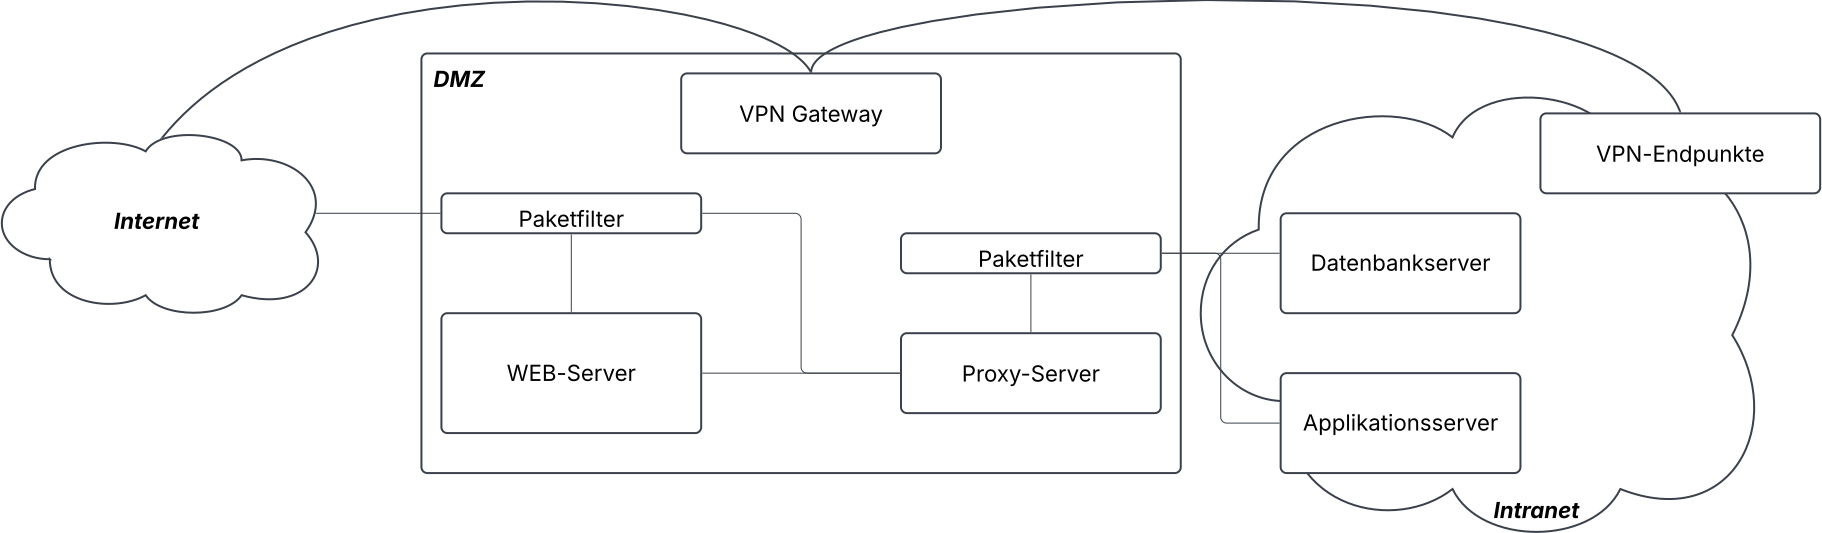
\includegraphics[scale=0.25]{aufgabe 2/img/screened_subnet.svg}
    \caption{Skizzierung der Sicherheitsarchitektur des Online-Händlers. (Quelle: eigene)}
    \label{fig:screened_subnet}
\end{figure}

\noindent
Nachfolgend geschaltete Proxy-Server und Paketfilter schützen das \textbf{innere Netz} des Betreibers nicht nur durch maliziöse Anfragen des \textbf{externen Netzes}, sondern auch vor Kompromittierten Systemen des Zwischennetzes (DMZ) sowie auch des inneren Netzes, in dem Weitere sensible Daten lagern: Anwendungsdaten und Artikeldaten des Onlineshops, aber auch Geschäftsdaten und Personaldaten.\\
Dem \textbf{innere Netz} muss dementsprechend Aufmerksamkeit zuteil werden, (Hardware-)Systeme müssen durch entsprechende Zugriffs- und Zugangskontrollen geschützt werden, Security-Policies müssen auf den Schutzbedarf der einzelnen Daten, die gespeichert bzw. über interne Telekommunikationsleitungen übertragen werden, geschützt werden.\\
Aus dem Schutzbedarf dieser Daten leitet sich dann ebenfalls das umzusetzende Sicherheitsniveau für das interne Netz ab, welches im gleichen Maße zu berücksichtigen ist, um ein insg. hohes Sicherheitsniveau zu erreichen.\\
Die angesprochenen \textbf{detektiven} Maßnahmen realisiert der Betreiber über spezielle (gesicherte) Loggingverfahren, die  \textbf{Intrusion Detection Systeme} unterstützen bzw. nachträglich bei evtl. forensischen Maßnahmen der Beweissicherung dienen, und aus denen weitere präventive Maßnahmen abgeleitet werden können.

\noindent
Sollten Mitarbeiter bzw. die Geschäftsleitung von Außen auf das innere Netz zugreifen müssen, ist der Einsatz von VPN dringend anzuraten. Beonders zu berücksichtigen ist die Tatsache, dass im inneren Netz auch die Datenbanken liegen, hier müssen also entsprechende Sicherheitsmaßnahmen zur Absicherung der KOmmunikation getroiffen werden.\\
Hierbei kann das VPN-Gateway innerhalb der DMZ liegen, oder es kann eine gesonderte DMZ nur für diesen Zweck aufgebaut werden, was möglicherweise die Sicherheit erhöht, gleichzeitig aber auch die \textbf{Komplexität} und den \textbf{Konfigurationsaufwand}.
Mitarbeiter müssen der im inneren Netz vorherrschenden Security Policy entsprechend geschult und bzgl. der möglichen Gefahren und Bedrohungen hin sensibilisiert werden.\\

\noindent
Der Betreiber muss überdies für die Identität seiner Server Sorge tragen, die mit Hilfe Dritter (\textit{Zertifizierungsstellen}, \textit{Trusted Authorities}) realisiert wird: Zusammen mit auf den Webservern installierten Software-Komponenten zur Verschlüsselung des Datenverkehrs (\textbf{HTTPS} mittels \textit{TLS}) wird die \textbf{Verschlüsselung} und \textbf{Signatur} der übertragenen Daten gewährleistet, wodurch die Sicherheitsziele \textbf{Vertraulichkeit} und \textbf{Verbindlichkeit} der Kommunikation sichergestellt wird.\\

\noindent
Das Abschicken von Bestellungen sollte ausschließlich über die Webanwendung erfolgen können.
Durch den Einsatz kryptografischer Maßnahmen wie HMAC und Signaturen unterstützt dies die Sicherstellung der Authentizität, aber auch Anwender erhalten durch entsprechend signierte Email-Antworten inkl. Rechnungen eine \textbf{verbindliche Auftragsbestätigung}.\\

\noindent
Zur Sicherstellung der Authentizität der Benutzer sind gesonderte Verfahren notwendig, wie bspw. Verifikation der eingegebenen Adressen bis hin zur Online-PIN bzw. Video-Ident-Verfahren. Diese müssen bereits bei der Anmeldung der Nutzer mit eingeplant werden.\\
Zusätzlich sollte der Betreiber dafür Sorge tragen, dass die Kreditkarteninformation gesichert auf seinen Servern gespeichert werden, beispielsweise unter Berücksichtigung des PCI-DSS (\textit{Payment Card Security Standard}, s.~\cite[57 ff.]{ITS1}).\\
Je nach Aufwand und Verhältnismäßigkeit bietet sich ein Auslagern des Zahlungsverkehrs an spezialisierte Dienstleister an bzw. die Einbettung von Verifikationsverfahren der zugehörigen Kreditsinstitute.\\

\noindent
Zur Absicherung von getätigten Bestellungen bzw. zur Einleitung von Bezahlvorgängen sollte die Identität und autoritative Nutzung der angegebenen Bezahldaten des Nutzers wiederholt sichergestellt werden, bspw. durch MFA-Verfahren.
Diese Maßnahmen sind auf Anwendungsebene zu treffen.

\subsection{Ablauf einer Bestellung}


\begin{itemize}
    \itemsep0.5em
    \item Öffnen der Webseite des Betreibers über gesicherte Verbdindung (HTTPS), Abgleich von Zertifikatsinformationen des Webservers mit der ausstellenden Zertifizieungsstelle, Abgleich öffentlicher / privater Schlüssel, Verifikation durch Webbrowser Nutzer / den Nutzer selber (wird in den weiteren Schritten bei der Kommunikation mit den Webservern/-diensten des Betreibers implizit vorausgesetzt)
    \item \textit{Neuer Nutzer}
    \begin{itemize}
        \item Registrierung des Nutzers über Online-Formular, Angabe von Adresse, MFA-Verfahren, ggf. Telefonnummer. Abgleich der Daten durch die Anwendung, ggfl. Abgleich Adressdatenbanken, White-/Blacklists Email-Adresse, Nutzername usw., Absenden Bestätigungsemail
        \item verifikation der Anmeldung durch den Nutzer (Double-Opt-In)
    \end{itemize}
    \item Anmeldung des Nutzers über Loginformular der Webseite, Bestätigung der Identität über MFA; Sitzung gesichert auf Anwendungsebene über verschlüsselte Tokens zur weiteren Kommunikation mit den Online-Diensten
    \item Auswahl der Artikel im Katalog des Händlers, Speicherung der ausgewählten Artikel im Warenkorb, Einleiten Bezahlvorgang
    \item Angabe der Zahlungsdaten, Auswahl nach Vorgabe des Betreibers. GGf. Möglichkeit zur Auswahl externer Dienstleister, optional speichern der Zahlart für nachfolgende Bestellvorgänge zur Vereinfachung des Bestellvorgangs. Abgleich der Daten durch externen Dienstleister und / oder Kreditsinstitute über gesicherte Verbindung, kryptografische Maßnahmen ähnlich zu dem beschriebenen System (Integrität / Authentizität Client - Server)
    \item Nach erfolgreicher Bestellung: Zusicherung der Verbindlichkeit der Bestellung durch Bestellbestätigung und Auftragseingang Online-Händler, Email entsprechend der Zertifizierungsmaßnahmen signiert und gehasht mit den privaten Schlüssel des Betreibers, Überprüfung durch Anwender/seinen Anwendungsprogrammen anhand des öffentlichen Schlüssel des Betreibers.
\end{itemize}